% Created 2018-12-29 sáb 20:59
\documentclass[a4paper, 12pt]{article}
\usepackage[utf8]{inputenc}
\usepackage[T1]{fontenc}
\usepackage{fixltx2e}
\usepackage{graphicx}
\usepackage{longtable}
\usepackage{float}
\usepackage{wrapfig}
\usepackage{rotating}
\usepackage[normalem]{ulem}
\usepackage{amsmath}
\usepackage{textcomp}
\usepackage{marvosym}
\usepackage{wasysym}
\usepackage{amssymb}
\usepackage{hyperref}
\tolerance=1000
\usepackage[left=3cm, right=3cm, top=3.5cm, bottom=3.5cm]{geometry} % Márgenes recomendados
\usepackage{times} % La fuente debe ser Times New Romans
\usepackage[english, spanish, es-noshorthands, es-tabla]{babel}
\usepackage[spanish]{translator}
\usepackage[style=ieee, backend=biber]{biblatex} % Bibliografía en formato IEEE
\usepackage{sectsty}
\usepackage{portada}
\usepackage[newfloat]{minted}
\usepackage{caption}
\newenvironment{code}{\captionsetup{type=listing}}{}
\SetupFloatingEnvironment{listing}{name={Fragmento de código},fileext=lol}
\setcounter{secnumdepth}{4}
\setcounter{tocdepth}{4}
\usepackage[titles]{tocloft}
\newlistof{listing}{lol}{Índice de ejemplos de código}
\sectionfont{\MakeUppercase} % Las secciones deben estar en mayúsculas
\bibliography{\jobname}
\Director{Fernando Pérez Costoya}
%\Lugar{Bilbao} % Por omisión: Madrid
%\Grado{Graduado en Matemáticas e Informática} % Por omisión: Graduado en Ingeniería Informática
%\Trabajo{TRABAJO FIN DE MÁSTER} % Por omisión: TRABAJO FIN DE GRADO
\author{Carlos Sánchez Marín}
\date{Enero de 2019}
\title{Desarrollo de una solución nativa y multiplataforma para la interacción desde una plataforma móvil con una aplicación bancaria}
\hypersetup{
  pdfkeywords={},
  pdfsubject={},
  pdfcreator={Emacs 25.2.2 (Org mode 8.2.10)}}
\begin{document}

\maketitle
\begin{export}
\null
\newpage

\pagenumbering{roman}
\tableofcontents
\newpage

\listoffigures
\listoftables
\listoflistings
\newpage
\end{export}

\begin{abstract}
\normalsize
Aquí el texto del abstract.

\textbf{Palabras clave:} palabra 1, palabra 2, palabra 3\ldots{}
\end{abstract}

\begin{otherlanguage}{english}
\begin{abstract}
\normalsize
Here goes the abstract text.

\textbf{Keywords:} keyword 1, keyword 2, keyword 3\ldots
\end{abstract}
\end{otherlanguage}

\newpage
\pagenumbering{arabic}% Iniciamos la numeración árabe en la primera sección

\section{Introducción}
\label{sec-1}
En los últimos años el sector bancario ha visto como los pagos con tarjetas ha crecido exponencialmente.
Según los datos ofrecidos por el Banco de España, desde 2002 hasta 2017 el número de operaciones creció
un 245\% y el importe de las operaciones un 188\%, llegando a un gasto total de 135.246,47 millones de €
en el 2017\cite{BancoEspana}.
\\
\\
Este rápido incremento de las operaciones con tarjeta también se ha trasladado al entorno corporativo,
generando nuevas necesidades para el control por parte de las empresas de las tarjetas que dan a sus
empleados. Con el objetivo de cubrir esta necesidad, tanto Mastercard \footnote{\url{https://developer.mastercard.com/product/spend-controls}} como Visa \footnote{\url{https://developer.visa.com/capabilities/vctc}} han
implementado nuevas funcionalidades de control de tarjetas que permiten el control directo por parte
de las empresas de sus tarjetas, de manera que se puedan recibir alertas de gasto o bloquear determinados tipos de pago.
\\
\\
Este servicio es ofrecido a través de diversas API REST y en Vipera hemos implementado una aplicación que
abstrae a los clientes finales (bancos y empresas) de las API proporcionadas por Visa y Mastercard,
ofreciendo una API REST centralizada que simplifica las operaciones. Esta API interactúa con un servicio
propietario de Vipera que integra toda la funcionalidad requerida por los distintos clientes finales.
\\
\\
Los SDK desarrollados para la integración de nuestro servicio en las aplicaciones móviles de los clientes
pretenden abstraer totalmente de las llamadas al servicio de manera que los desarrolladores tan solo
vean funciones totalmente descriptivas sin tener que preocuparse de la configuración necesaria para la
interacción. Así mismo, ya que la demo técnica realizada por Vipera está implementada con Ionic\footnote{\url{https://ionicframework.com/}},
se ha implementado un plugin de Cordova\footnote{\url{https://cordova.apache.org/}} que habilita la llamada a los SDK de iOS y Android.

\section{Estado del arte}
\label{sec-2}
\subsection{Tecnologías}
\label{sec-2-1}
En el mercado móvil actual iOS y Android lideran con mano de hierro dejando una cuota residual a otros
entornos como Windows Phone y otros sistemas menores. En conjunto, iOS y Android acapararon el 99,7\% de
las ventas en el primer trimestre de 2018 en España, dejando a Windows fuera de las estadísticas al no lograr
el 0,1\% de las ventas totales\footnote{\url{https://bit.ly/2Cu8NVy}}. Teniendo presentes estos datos, resulta obvio que cualquier tipo de desarrollo
fuera de Android e iOS tendría un impacto muy reducido y difícilmente sería rentable para cualquier aplicación
que no tenga como objetivo a todos los usuarios del mercado móvil.
\subsubsection{iOS}
\label{sec-2-1-1}
El sistema operativo iOS es un sistema propietario desarrollado por Apple\footnote{\url{https://apple.com/es/}} para sus dispositivos
móviles iPhone, iPad y iPod Touch. Fue presentado junto con el primer iPhone en junio de 2007. En un
principio Apple no iba a proporcionar SDK para desarrollo de aplicaciones nativas por parte de terceros,
pero ante la reacción negativa de todos los desarrolladores, Apple reconsideró su decisión y terminó
lanzando la primera versión del SDK en Marzo de 2008 junto a la segunda versión de iOS.
\\
\\
El SDK originalmente proporcionaba un acceso muy limitado a las funciones del sistema operativo,
además de tan solo proporcionar soporte para el lenguaje Objective-C\footnote{\url{https://developer.apple.com/library/archive/documentation/Cocoa/Conceptual/ProgrammingWithObjectiveC/Introduction/Introduction.html}}. Año tras año Apple ha
actualizado su sistema operativo móvil junto con el SDK aprovechando el lanzamiento de los nuevos iPhone.
\\
\\
En 2014, Apple lanzó Swift\footnote{\url{https://swift.org/}}, un nuevo lenguaje más moderno que sustituyó a Objective-C como
lenguaje de referencia para el desarrollo de aplicaciones iOS. No obstante, ambos lenguajes son actualmente
soportados por el SDK de Apple, aunque la documentación tan solo es actualizada para Swift.
\\
\\
\subsubsection{Android}
\label{sec-2-1-2}
Android\footnote{\url{https://www.android.com}} fue creado en 2003 como un fork del kernel de Linux para dispositivos
móviles. Inicialmente fue concebido como un sistema operativo móvil inteligente que
estuviese pendiente de la localización del usuario y sus preferencias. En 2005 la
empresa propietaria del sistema operativo fue comprada por Google, que se hizo cargo
del desarrollo. Dos años más tarde, Google hizo público el primer SDK en fase beta
para Android, que fue distribuido a desarrolladores y fabricantes de dispositivos
móviles. No fue hasta septiembre de 2008 que se lanzó al mercado el primer dispositivo
con Android.
\\
\\
Las primeras versiones del SDK proporcionado por Google contaban tan solo con
soporte para el lenguaje Java\footnote{\url{https://www.java.com}}. Al contrario de su principal competidor, el código fuente
de Android siempre ha sido open source\footnote{\url{https://source.android.com/}} lo que ha atraído a una gran cantidad de
desarrolladores y fabricantes. De todos modos, la práctica totalidad de los fabricantes
integran en sus terminales la versión de Android propietaria de Google, que incluye
integración con las apps de Google bajo la capa Google Play Services\footnote{\url{https://developers.google.com/android/guides/overview}}.
\\
\\
En el evento Google I/O de 2017, Google anunció de manera oficial que se añadía un
nuevo lenguaje soportado al SDK de Android \footnote{\url{https://blog.jetbrains.com/kotlin/2017/05/kotlin-on-android-now-official/}}, Kotlin\footnote{\url{https://kotlinlang.org/}}. Este lenguaje desarrollado
por la empresa Jetbrains\footnote{\url{https://www.jetbrains.com/}} funciona sobre la Java Virtual Machine, por lo que es totalmente compatible con el código Java y puede
coexistir con este en una misma aplicación.
\subsubsection{Cordova}
\label{sec-2-1-3}
En el año 2011, Adobe Systems\footnote{\url{https://www.adobe.com/}} compró la empresa Nitobi y renombró su producto
como Phonegap\footnote{\url{https://phonegap.com/}} . Así mismo, lanzó una versión open source del producto nombrada
Cordova que es mantenida por la Apache Software Foundation\footnote{\url{https://www.apache.org/}}.
Este framework permite el desarrollo de aplicaciones híbridas basadas en la web,
embebiendo una aplicación web dentro de una aplicación nativa para el sistema
operativo deseado. Esta solución se acerca a la idea que tenía Apple de aplicaciones
móviles en un principio, pero va más allá otorgando un sistema de plugins nativos que
permiten la interacción con el sistema operativo.
\\
\\
Los plugins proporcionan una implementación en código nativo (Objective-C para iOS
y Java para Android) que será invocada por un wrapper escrito en Javascript\footnote{\url{https://developer.mozilla.org/bm/docs/Web/JavaScript}}. En
tiempo de ejecución Cordova es capaz de saber sobre qué plataforma está ejecutándose
e invocar al código nativo de esta, con lo que abstrae a los desarrolladores de
aplicaciones de esta gestión y facilita la escritura de código.
\subsection{MOTIF}
\label{sec-2-2}
El despliegue del lado del servidor de la aplicación bancaria con la que se ha operado
para la realización de este trabajo está realizado sobre una plataforma propietaria propiedad
de Vipera\footnote{\url{http://www.vipera.com/}} cuyo nombre comercial es MOTIF\footnote{\url{http://www.vipera.com/motif}}.
\\
\\
MOTIF es un servicio desarrollado en Java haciendo uso del framework OSGi\footnote{\url{https://www.osgi.org/}}, creado en 1999
como una primera aproximación al mundo de los microservicios en Java. En concreto, el desarrollo de MOTIF
ha sido llevado a cabo empleando Apache Felix\footnote{\url{https://felix.apache.org/}} como implementación del framework OSGi. El uso de
este framework facilita la integración con los clientes finales, por lo general banco y otros servicios
financieros, ya que estos suelen emplear Java en sus propios servicios y la arquitectura OSGi permite una
integración sencilla de diferentes módulos a los que se llama \emph{plugins} con el resto del sistema. En la \hyperref[fig:motif-core]{figura 1}
se representan los servicios básicos implementados en el core de MOTIF.
\begin{figure}[htb]
\centering
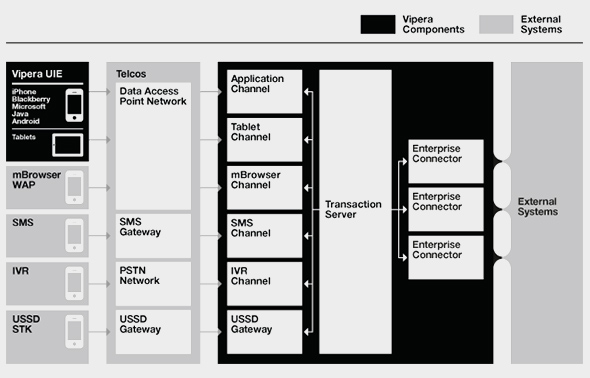
\includegraphics[width=.9\linewidth]{./images/motif.jpg}
\caption{\label{fig:motif-core}Diagrama de módulos predefinidos de MOTIF}
\end{figure}
\\
\\
En el caso concreto de la aplicación para la que se ha implentado la solución desarrollada como trabajo
fin de grado, se ha hecho uso de los plugins que conforman el core de MOTIF, además de distintos plugins que
permiten la interacción con los servicios de Mastercard y VISA, así como plugins de persistencia de datos empleando
la librería Hibernate\footnote{\url{https://hibernate.org/}} y otros que implementan toda la lógica de negocio, que será explicada más adelante.
\\
\\
Para realizar la conexión con MOTIF, por defecto existen 2 métodos distintos:
\begin{itemize}
\item \textbf{API REST}: Está pensada para dar servicio a implementaciones de administracióndel sistema como podría ser un Help Desk.
\item \textbf{JSON Protocol}: Este método de conexión es el que se emplea en las soluciones móviles. Se basa en peticiones POST a un endpoint estático, el cual procesa la información enviada en la petición y determina el comportamiento que debe seguir el servidor.
\end{itemize}

\subsection{Modos de conexión con MOTIF desde una aplicación móvil}
\label{sec-2-3}
\subsubsection{Peticiones POST}
\label{sec-2-3-1}
La forma más básica de hacer llamadas al endpoint JSON de MOTIF es la construcción de peticiones POST haciendo uso
de aplicaciones como Postman\footnote{\url{https://www.getpostman.com/}} o empleando directamente las librerías HTTP de los distintos lenguajes.
El siguiente \hyperref[code:jsonmotif]{JSON} es un ejemplo del cuerpo de una llamada a MOTIF.
\\
\begin{code}
\label{code:jsonmotif}
\begin{minted}[linenos,tabsize=2,breaklines]{json}
{
  "req" : {
        "dom" : "{{domain}}",
        "app" : "{{application}}",
        "srv" : "{{service}}",
        "op"  : "{{operation}}",
        "header" :
        {
            "user":"user1@company1.com",
            "otp":"123456",
            "private:pwd":"1111",
            "private:vpwd":"1111",
            "email": "user1@company1.com"
        }
    }
}
\end{minted}
\captionof{listing}{Cuerpo de una petición POST a MOTIF}
\end{code}
\bigbreak
\\
Como se puede apreciar, todos los campos de la llamada están encapsulados dentro del parámetro \emph{req}, el cual
es interceptado por el endpoint JSON de MOTIF. Una vez se ha interceptado la llamada, MOTIF comprueba los campos
\emph{dom} (dominio al que se está llamando), \emph{app} (aplicación del dominio), \emph{srv} (servicio de la aplicación) y \emph{op}
(operación del servicio).
\\
\\
Por último, en el campo \emph{header} se encontrarán contenidos los parametros requeridos por la operación. En este caso
se trata de una llamada de ejemplo para la activación de usuarios, por lo que se pasan como parámetros el usuario,
OTP (One Time Password), contraseña y su verificación y el email del usuario. Cabe destacar que los campos ligados a
la contraseña tienen el prefijo \emph{private}, el cual al ser detectado por MOTIF le indica que no debe quedar constancia
en los logs de esos campos.
\subsubsection{Motif Connector}
\label{sec-2-3-2}
Uno de los equipos de desarrollo de Italia implementó una librería para abstraer de ciertos detalles a los desarrolladores
de las aplicaciones móviles que emplean como backend MOTIF. Esta librería fue implementada tanto en Objective-C para iOS
como en Java para Android. También se implementó un plugin de Cordova para facilitar su uso en aplicaciones híbridas.
\\
\\
En el siguiente \hyperref[code:motifconnector]{código} podemos observar como se compone la misma llamada a MOTIF expuesta en
el apartado anterior empleando el plugin para Cordova. Podemos observar el campo \emph{header} sigue existiendo y siendo definido
como un JSON, pero el usuario queda abstraido del formato del JSON que configura el dominio, aplicación, servicio y operación.
\\
\\
Por último, se puede observar en la composición de la llamada al servidor que hay un campo booleano marcado como \emph{false}. Este
campo determina si la llamada es segura, lo que implicaría la necesidad de que en la llamada incluya un ID de sesión para el
usuario que la hace. El plugin implementa una función que guarda en la instancia este ID una vez el usuario se autentica con el
servido. En este caso la llamada es de activación de un usuario, por lo que no se puede tener un ID de sesión.
\begin{code}
\label{code:motifconnector}
\begin{minted}[linenos,tabsize=2,breaklines]{ts}
let myHeader = {
        "user":"user1@company1.com",
        "otp":"123456",
        "private:pwd":"1111",
        "private:vpwd":"1111",
        "email": "user1@company1.com"
      };

      let request: MotifRequest = this.motifClient.buildServerRequest("register", "activateUser", myHeader, false);

      this.motifClient.sendRequest(request).then((res: MotifResponse) => {
        /*Codigo a ejecutar en caso de exito*/
      },(err) => {
        /*Codigo a ejecutar en caso de error*/
      });
\end{minted}
\captionof{listing}{Ejemplo de una llamada empleando el plugin Motif Connector}
\end{code}
\bigbreak
Esta libreria es la que se emplea como base para todas las soluciones personalizadas ofrecidas por Vipera, incluyendo la solución
expuesta en este documento.
\subsection{Card Control}
\label{sec-2-4}
En verano de 2017 se implementó un prototipo para Deutsche Bank en colaboración con Mastercard, que implementaba una solución parecida
a la desarrollada para \hyperref[sec:smepay]{SME Pay}, pero sin ofrecer la opción del control de tarjetas empresariales. Esta solución fue desplegada con éxito
y ha sido usada como base de la lógica de negocio del proyecto SME Pay.
\section{SME Pay}
\label{sec-3}
\label{sec:smepay}
La solución implementada forma parte del proyecto SME Pay\footnote{\url{http://www.vipera.com/sme-pay-2/}}, un proyecto iniciado en colaboración con Mastercard para el control
de gastos efectuado con tarjetas de empresa. En la actualidad el producto también ofrece la misma funcionalidad para tarjetas de VISA,
siendo la gestión totalmente indiferente de cara al usuario, ya que las diferencias entre los distintos entornos son manejadas internamente
por MOTIF.
\subsection{Estructura de la aplicación}
\label{sec-3-1}
En la actualidad SME Pay ofrece 2 areas diferenciadas claramente. Por un lado se proporciona la posibilidad de controlar tarjetas personales,
que podrán ser añadidas y eliminadas de manera arbitraria por cada usuario y a las que ningún otro usuario que no sea el propietario podrá tener
acceso. Por otro lado, los gestores de las empresas que adquieran el producto tendrán acceso desde su aplicación a un apartado diferenciado que
permitirá controlar las tarjetas de la empresa. Para efectuar este control se han implementado distintos servicios que interactuan entre ellos
tal y como se puede observar en la \hyperref[fig:sme-services]{figura 2}.
\begin{figure}[htb]
\centering
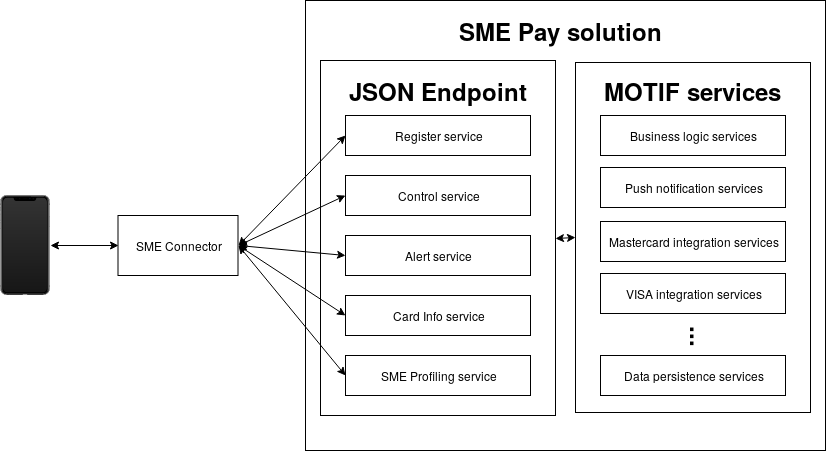
\includegraphics[width=.9\linewidth]{./images/smepay.png}
\caption{\label{fig:sme-services}Servicios proporcionados por el JSON Endpoint de SME Pay}
\end{figure}
\subsubsection{Servicio \emph{register}}
\label{sec-3-1-1}
El servicio register ofrece funcionalidades de activación, login y logout. Para efectuar un login se puede hacer tanto empleando el PIN elegido por el usuario como su huella dactilar en caso de que el
dispositivo móvil permita, así como el uso de la tecnología de reconocimiento facial en los modelos de Apple que así lo permitan.
\subsubsection{Servicio \emph{alert}}
\label{sec-3-1-2}
El servicio alert gestiona la configuración de notificaciones de las tarjetas personales de cada usuario. Tal y como se puede observar en la \hyperref[fig:trx-alert]{figura 3}
en este punto debemos diferenciar entre notificaciones de los servicios ofrecidos por Mastercard y VISA y las notificaciones push que manda SME Pay a
los terminales móviles de los usuarios.
\\
\\
Por un lado SME Pay configura todas las tarjetas registradas con Mastercard y VISA para recibir notificaciones de cualquier operación realizada. Sin embargo,
los usuarios tienen la capacidad de configurar a través de este servicio que notificaciones push quieren recibir (retirada de dinero de un cajero, pagos online,
operaciones por encima de un límite marcado\ldots{}). De este modo el usuario tiene la libertad de gestionar las notificaciones que recibe en su dispositivo y al mismo
tiempo el banco o empresa que contrata el servicio SME Pay tiene un registro accesible de todas las tarjetas registradas.
\begin{figure}[htb]
\centering
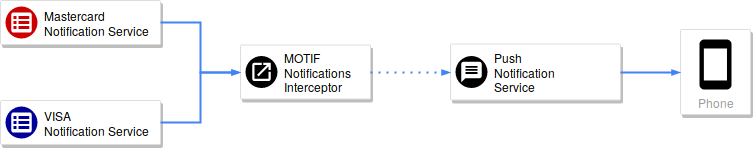
\includegraphics[width=.9\linewidth]{./images/Trx-notification.png}
\caption{\label{fig:trx-alert}Diagrama de funcionamiento de notificaciones en SME Pay}
\end{figure}
\subsubsection{Servicio \emph{control}}
\label{sec-3-1-3}
El servicio control gestiona los bloqueos que se pueden establecer sobre las tarjetas personales de cada usuario.
\subsubsection{Servicio \emph{cardinfo}}
\label{sec-3-1-4}
El servicio cardinfo ofrece funcionalidades de registro, activacion, desactivación y eliminación de tarjetas, así como también facilita las tarjetas registradas
por el usuario y sus transacciones asociadas almacenadas en los servidores de SME Pay.
\subsubsection{Servicio \emph{smeprofiling}}
\label{sec-3-1-5}
El servicio smeprofiling es el principal del producto SME Pay. Este proporciona las mismas funcionalidades que los servicios \emph{alert},/control/ y \emph{cardinfo} añadiendo toda la lógica de negocio necesaria
para permitir la gestión de las tarjetas de empresa tanto por los usuarios que las tienen asignadas, como por los gestores. En SME Pay se diferencia entre 3 tipos de usuarios: \hyperref[sec:bsowner]{Business owner}, \hyperref[sec:gadmin]{Group Admin}
y \hyperref[sec:user]{User}.
\paragraph{Business Owner}
\label{sec-3-1-5-1}
\label{sec:bsowner}
El business owner es el usuario que tiene todos los permisos posibles dentro de la escala de privilegios establecida en SME Pay. Puede configurar las notificaciones push para las tarjetas
de compañía de forma que le lleguen notificaciones de todas las tarjetas o notificaciones de tarjetas de grupos concretos.
\\
\\
Respecto a los distintos bloqueos que pueden realizarse sobre las tarjetas, también puede establecer un bloqueo sobre todas las tarjetas de la compañía o sobre las tarjetas de un grupo concreto. Cuando
establece estos bloqueos, todas las tarjetas afectadas deshabilitan la gestión de dicho bloqueo al resto de usuarios.
\paragraph{Group Admin}
\label{sec-3-1-5-2}
\label{sec:gadmin}
El business owner puede establecer un group admin para cada uno de los grupos que decida crear. Estos group admin podrán configurar las notificaciones push para las tarjetas de su propio grupo.
Por otro lado, también tendrán la capacidad de establacer bloqueos en las tarjetas del grupo siempre y cuando el business owner no lo haya hecho antes.
\paragraph{User}
\label{sec-3-1-5-3}
\label{sec:user}
Todos los usuarios de SME Pay tiene por defecto privilegios de user. Pueden configurar notificaciones para la tarjeta de compañía que les ha sido asignada y bloqueos, siempre y cuando no hayan sido
establecidos por el business owner o el group admin.

\subsection{Interacción con SME Pay}
\label{sec-3-2}
\subsubsection{Aplicación de Vipera}
\label{sec-3-2-1}
Para la presentación del producto SME Pay en el Finovate London 2018\footnote{\url{https://finovate.com/videos/finovateeurope-2018-vipera-mastercard/}} se desarrolló un prototipo de aplicación móvil en Ionic que conectaba con el producto mediante llamadas HTTP realizadas directamente por
el módulo http del core de Angular.
\begin{code}
\label{code:angularhttp}
\begin{minted}[linenos,tabsize=2,breaklines]{ts}
let headers = new HttpHeaders();
      headers = headers.set('Content-Type', 'application/json');

        this.http.post(ENV.serverUrl, {
          "req": {
            "dom": ENV.domain,
            "app": ENV.application,
            "srv": "register",
            "op": "activateUser",
            "header": {
              "user": this.regForm.value.user,
              "email": this.regForm.value.email,
              "otp": this.regForm.value.otp,
              "private:pwd": this.regForm.value.password,
              "private:vpwd": this.regForm.value.verify,
            }
          }
        },
        {headers: headers})
        .subscribe(
          res => {
            if(res["res"]["header"]["err"] != undefined) {
              /*Codigo a ejecutar en caso de error*/
            } else {
              /*Codigo a ejecutar en caso de exito*/
            }
          });
\end{minted}
\captionof{listing}{Llamada a la operación activation del servicio register empleando el cliente HTTP}
\end{code}
\bigbreak
Este método de conexión a pesar de ser completamente funcional, requería muchas lineas de código, lo que generaba un código muy denso y costoso de mantener. Por este motivo, tras el interes de
diversos potenciales clientes se decidió integrar la librería MOTIF Connector, con lo que él código se reduce notablemente \hyperref[code:motifconnector]{(ver Fragmento de código 2)}.
\subsubsection{Integración en aplicaciones de terceros}
\label{sec-3-2-2}
Dado que los potenciales clientes objetivo de SME Pay son bancos y PYMES, se decidió desarrollar unas librerías nativas para Android e iOS y adicionalmente un plugin de Cordova, con lo que se facilita
a los clientes la integración del producto en sus aplicaciones móviles ya funcionales, con una abstracción total de la interacción con MOTIF.
\section{Desarrollo de la solución}
\label{sec-4}
\subsection{Desarrollo de la librería para Android}
\label{sec-4-1}
\subsubsection{Estructura del proyecto}
\label{sec-4-1-1}
El proyecto cuenta en su raiz con un fichero de configuracion para Gradle\footnote{\url{https://gradle.org/}}, herramienta utilizada para construir la librería.
\\
El código se encuentra distribuido en 2 partes. Por un lado se implementan las clases que establecen la conexión con el servidor y tratan las respuestas. En el caso de Java, ya que este no contempla
el uso de funciones de callback en la versión 1.7, se ha desarrollado para cada clase una interfaz asociada que será la que implemente cada función para emplearla de callback.
\bigbreak
\begin{code}
\label{code:androidcallback}
\begin{minted}[linenos,tabsize=2,breaklines]{java}
public interface RegisterServiceCallback<T> {
    /**
     * method invoked when an {@link IRegisterService} api is successfully done
     * @param result api result
     */
    void onSuccess(T result);

    /**
     * method invoked when an {@link IRegisterService} api is done with an error
     * @param error the error
     */
    void onError(IDEError error);
}
\end{minted}
\captionof{listing}{Implementación de una interfaz de callback para el servicio register}
\end{code}
\bigbreak
Por otro lado, se encuentra el código encargado de serializar y deserializar las llamadas y respuestas del servidor.
\subsection{Desarrollo de la libreria para iOS}
\label{sec-4-2}
\subsubsection{Estructura del proyecto}
\label{sec-4-2-1}
El proyecto está estructurado en 2 partes. Por un lado se encuentra todo el código referente a los servicios de SME Pay, donde se establece la conexión con el servidor y se tratan las respuestas.
\\
Por otro lado, se encuentra el código encargado de serializar y deserializar las llamadas y respuestas del servidor.
\\
Por último, en la raiz del proyecto se encuentra el fichero \verb~DECardControl.h~, que expone todas las cabeceras públicas de la librería para posibilitar su uso por parte de los desarrolladores.
\subsubsection{Serialización y deserialización}
\label{sec-4-2-2}
Debido a que Objective-C no ofrece soporte nativo para JSON, se necesita implementar clases que se encarguen de serializar y deserializar. Esto se consigue empleando la estructura de datos \verb~NSDictionay~
que como su nombre indica es un diccionario.
\\
\\
La estructura de estas clases es muy sencillo, tan solo tienen un constructor al que se le pasan todos los parametros a serializar y dos métodos, para serializar y deserializar. También se tiene que definir
estáticamente el nombre de los campos del JSON, de forma que estos se usen como las \emph{key} del diccionario.
\begin{code}
\label{code:ios-serializer}
\begin{minted}[linenos,tabsize=2,breaklines]{obj-c}
//
//  DEActivateUserRequest.m
//  DECardControl
//
//  Created by SME Project Team on 03/10/18.
//  Copyright © 2018 Vipera. All rights reserved.
//

#import "DEActivateUserRequest.h"

#define DE_ACTIVATE_REQUEST_KEY_USER @"user"
#define DE_ACTIVATE_REQUEST_KEY_EMAIL @"email"
#define DE_ACTIVATE_REQUEST_KEY_OTP @"otp"
#define DE_ACTIVATE_REQUEST_KEY_PASSWORD @"private:pwd"
#define DE_ACTIVATE_REQUEST_KEY_VPASSWORD @"private:vpwd"

@interface DEActivateUserRequest ()

@property (nonatomic, strong, readwrite) NSString *userID;
@property (nonatomic, strong, readwrite) NSString *email;
@property (nonatomic, strong, readwrite) NSString *otp;
@property (nonatomic, strong, readwrite) NSString *password;
@property (nonatomic, strong, readwrite) NSString *vPassword;

@end

@implementation DEActivateUserRequest

+ (instancetype)initWithDictionary:(NSDictionary *)dictionary error:(NSError *__autoreleasing *)error
{
    NSString *userID = dictionary[DE_ACTIVATE_REQUEST_KEY_USER];
    NSString *email = dictionary[DE_ACTIVATE_REQUEST_KEY_EMAIL];
    NSString *otp = dictionary[DE_ACTIVATE_REQUEST_KEY_OTP];
    NSString *password = dictionary[DE_ACTIVATE_REQUEST_KEY_PASSWORD];
    NSString *vPassword = dictionary[DE_ACTIVATE_REQUEST_KEY_VPASSWORD];

    return [[DEActivateUserRequest alloc] initWithUserID:userID email:email otp:otp password:password vPassword:vPassword];
}

- (instancetype) initWithUserID:(NSString *) userID
                          email:(NSString *) email
                            otp:(NSString *) otp
                       password:(NSString *) password
                      vPassword:(NSString *) vPassword
{
    self = [super init];

    if (self)
    {
        self.userID = userID;
        self.email = email;
        self.otp = otp;
        self.password = password;
        self.vPassword = vPassword;
    }

    return self;
}

- (NSDictionary *)toDictionary:(NSError *__autoreleasing *)error
{
    NSMutableDictionary *resultDictionary = [NSMutableDictionary dictionary];

    resultDictionary[DE_ACTIVATE_REQUEST_KEY_USER] = self.userID;
    resultDictionary[DE_ACTIVATE_REQUEST_KEY_EMAIL] = self.email;
    resultDictionary[DE_ACTIVATE_REQUEST_KEY_OTP] = self.otp;
    resultDictionary[DE_ACTIVATE_REQUEST_KEY_PASSWORD] = self.password;
    resultDictionary[DE_ACTIVATE_REQUEST_KEY_VPASSWORD] = self.vPassword;

    return resultDictionary;
}

@end

\end{minted}
\captionof{listing}{Implementación de una clase de serialización/deserialización en Objective-C}
\end{code}
\bigbreak
\subsubsection{Desarrollo de un servicio}
\label{sec-4-2-3}
Para proceder a un desarrollo de una librería coherente con la estructura de SME Pay, se decidió diferenciar cada servicio de la misma forma. Así mismo, cada servicio contará con 3 ficheros.
\paragraph{Interfaz del servicio}
\label{sec-4-2-3-1}
Este fichero actuará como interfaz pública del servicio, proporcionando todos los métodos que proporciona el servicio, definiendo los tipos que empleará para el tratamiento de las respuestas y
especificando que clases empleará para la serialización y deserialización de las llamadas y respuestas.
\begin{code}
\label{code:ios-interface-partial}
\begin{minted}[linenos,tabsize=2,breaklines]{obj-c}
//
//  IDELoginService.h
//  DECardControl
//
//  Created by SME Project Team on 02/10/2018.
//  Copyright © 2018 Vipera. All rights reserved.
//

#import <Foundation/Foundation.h>
#import "IDEError.h"

@class DELoginRequest, DELoginResponse, DEActivateUserRequest, DEChangePwdRequest, DEEnableFingerprintRequest, DEEnableFingerprintResponse, DELoginFingerprintRequest;

/**
 * Block invoked when a IDELoginService method has been failed
 **/
typedef void(^DELoginServiceFailure)(id<IDEError> error);

...

/**
 * Block invoked when the activateUser (@see -activateUserWithSuccess:successBlock :failureBlock) method was successful
 **/
typedef void (^DELoginServiceActivateUserSuccess)();

...

/**
 *
 *  @param successBlock The block invoked when the user activation has been successfully
 *  @param failureBlock The block invoked when the user activation has been failed
 */
- (void) activateUserRequest:(DEActivateUserRequest*) activateRequest successBlock:(DELoginServiceActivateUserSuccess) successBlock failure:(DELoginServiceFailure) failureBlock;

...

\end{minted}
\captionof{listing}{Implementación parcial de la interfaz del servicio register para la librería de iOS}
\end{code}
\bigbreak
Dado que la implementación completa es muy extensa, ha sido añadida en el \hyperref[code:ios-interface]{Anexo A}, dejando en esta parte del documento tan solo la implementación relativa a la llamada
\emph{activateUser}.
\paragraph{Implementación del servicio}
\label{sec-4-2-3-2}
Dado que Objective-C es un lenguaje basado en C, emplea la misma estructura para definir librerías. Por un lado se encuentra la cabecera que mantiene
la extensión \verb~<file>.h~ y por otro la implementación, que en este caso si cambia su extensión a \verb~<file>.m~.
\begin{code}
\label{code:ios-implementation}
\begin{minted}[linenos,tabsize=2,breaklines]{obj-c}
//
//  DELoginService.m
//  DECardControl
//
//  Created by SME Project Team on 02/10/2018.
//  Copyright © 2018 Vipera. All rights reserved.
//

...

#import "DEActivateUserRequest.h"

...

#import "DEMotifRequest.h"
#import "DEMotifResponse.h"
#import "DEError.h"

...

#define LOGIN_SERVICE_OP_ACTIVATE_USER @"activateUser"

...

@interface DELoginService ()

@end

@implementation DELoginService

...

- (void) activateUserRequest:(DEActivateUserRequest *)activateRequest successBlock:(DELoginServiceActivateUserSuccess)successBlock failure:(DELoginServiceFailure)failureBlock
{
    NSError *error = nil;
    NSDictionary *activationDictionary = [activateRequest toDictionary:&error];

    if (error)
    {
        failureBlock([DEError buildErrorWithError:error]);
        return;
    }

    DEMotifRequest *request = [self.serverManager buildRequestForService:LOGIN_SERVICE operation:LOGIN_SERVICE_OP_ACTIVATE_USER isSecure:NO];

    [request setHeader:activationDictionary];

    [self.serverManager postRequest:request successBlock:^(DEMotifResponse *successResult, DEMotifRequest *serverRequest) {
        successBlock();
    } motifErroBlock:^(DEMotifResponse *failureResult, DEMotifRequest *motifRequest) {
        failureBlock([DEError buildErrorWithMotifResponse:failureResult]);
    } failureBlock:^(NSError *error, DEMotifRequest *motifRequest) {
        failureBlock([DEError buildErrorWithError:error]);
    }];
}

...

@end

\end{minted}
\captionof{listing}{Código parcial de la implementación del servicio register para la librería de iOS}
\end{code}
\bigbreak
Debido a que el \hyperref[code:ios-implementation]{código} de la implementación de los servicios se proporciona compilado, tan solo se muestra la implementación de la llamada a la operación \emph{activateUser},
para seguir el mismo ejemplo empleado durante el documento. Todas las llamadas siguen el mismo patrón de todos modos. En primer lugar se serializan los datos de la llamada a MOTIF, contemplando el caso en
el que la serialización falle, de modo que se interrumpiría la ejecución. En caso de que la serialización se produzca con éxito, se realiza la llamada a MOTIF y se procesa la respuestá mediante el uso de
funciones inline.
\\
\\
En el caso de la operación \emph{activateUser} no se recibe ningún tipo de información que deba ser deserializada, pero en el caso de las operaciones en lo que esto si ocurre, se deserializa en en la función inline
correspondiente al éxito de la llamada, y se devuelve el objeto deserializado dentro del método \verb~successBlock()~.
\subsection{Desarrollo del plugin para Cordova}
\label{sec-4-3}
\subsubsection{Estructura del proyecto}
\label{sec-4-3-1}
Un plugin para Cordova tiene una estructura definida que puede ser encontrada en su documentación online\cite{Cordova}. Tal y como se indica, en la raiz del proyecto existe el fichero \hyperref[code:pluginxml]{plugin.xml},
el cual proporciona información acerca del plugin (nombre, versionado, licencia\ldots{}) y su composición interna. Este archivo es crucial ya que es el que lee Cordova al realizar la instalación de un plugin,
con lo que un error puede provocar un mal funcionamiento del plugin.
\begin{code}
\label{code:pluginxml}
\begin{minted}[linenos,tabsize=2,breaklines]{xml}
<plugin id="de-smepay-plugin" version="0.0.1" xmlns="http://apache.org/cordova/ns/plugins/1.0" xmlns:android="http://schemas.android.com/apk/res/android">
  <name>SMEPayConnector</name>

  <js-module src="www/CardControl.js" name="CardControl">
    <clobbers target="DynamicEngine.plugins.CardControl"/>
  </js-module>
  <js-module src="www/LoginService.js" name="LoginService">
    <clobbers target="DynamicEngine.plugins.CardControl.LoginService"/>
  </js-module>
  <js-module src="www/CardInfoService.js" name="CardInfoService">
    <clobbers target="DynamicEngine.plugins.CardControl.CardInfoService"/>
  </js-module>
  <js-module src="www/ControlService.js" name="ControlService">
    <clobbers target="DynamicEngine.plugins.CardControl.ControlService"/>
  </js-module>
  <js-module src="www/AlertService.js" name="AlertService">
    <clobbers target="DynamicEngine.plugins.CardControl.AlertService"/>
  </js-module>
  <js-module src="www/VirtualCardService.js" name="VirtualCardService">
    <clobbers target="DynamicEngine.plugins.CardControl.VirtualCardService"/>
  </js-module>
  <js-module src="www/SMEProfilingService.js" name="SMEProfilingService">
    <clobbers target="DynamicEngine.plugins.CardControl.SMEProfilingService"/>
  </js-module>

  <platform name="android">

    ...

    <source-file src="src/android/CardControlPlugin.java" target-dir="src/com/vipera/cardcontrolplugin" />
    <source-file src="src/android/AlertServicePlugin.java" target-dir="src/com/vipera/cardcontrolplugin" />
    <source-file src="src/android/CardInfoServicePlugin.java" target-dir="src/com/vipera/cardcontrolplugin" />
    <source-file src="src/android/ControlServicePlugin.java" target-dir="src/com/vipera/cardcontrolplugin" />
    <source-file src="src/android/LoginServicePlugin.java" target-dir="src/com/vipera/cardcontrolplugin" />
    <source-file src="src/android/VirtualCardServicePlugin.java" target-dir="src/com/vipera/cardcontrolplugin" />
    <source-file src="src/android/CardControlServicesProvider.java" target-dir="src/com/vipera/cardcontrolplugin" />
    <source-file src="src/android/SMEProfilingServicePlugin.java" target-dir="src/com/vipera/cardcontrolplugin" />
    <source-file src="src/android/Encode.java" target-dir="src/com/vipera/cardcontrolplugin" />
    <framework custom="true" src="src/android/SMEPay.gradle" type="gradleReference" />

  </platform>


  <platform name="ios">

    ...

    <framework src="src/ios/SMEPay.framework" custom="true" embed="true"/>

    <header-file src="src/ios/AlertServicePlugin.h" />
    <source-file src="src/ios/AlertServicePlugin.m" />
    <header-file src="src/ios/CardControlPlugin.h" />
    <source-file src="src/ios/CardControlPlugin.m" />
    <header-file src="src/ios/CardInfoServicePlugin.h" />
    <source-file src="src/ios/CardInfoServicePlugin.m" />
    <header-file src="src/ios/ControlServicePlugin.h" />
    <source-file src="src/ios/ControlServicePlugin.m" />
    <header-file src="src/ios/LoginServicePlugin.h" />
    <source-file src="src/ios/LoginServicePlugin.m" />
    <header-file src="src/ios/SmeProfilingServicePlugin.h" />
    <source-file src="src/ios/SmeProfilingServicePlugin.m" />
    <header-file src="src/ios/CardControlConfig.h" />
    <source-file src="src/ios/CardControlConfig.m" />
    <header-file src="src/ios/MotifConnectorConfiguration.h" />
    <source-file src="src/ios/MotifConnectorConfiguration.m" />

  </platform>

</plugin>
\end{minted}
\captionof{listing}{Código parcial del fichero plugin.xml del plugin}
\end{code}
\bigbreak
Como se puede observar en el código, cada plataforma para la que se ofrece soporte se configura de manera explicita, indicando los ficheros y su ubicación. Estos ficheros realizan llamadas a las librerías
nativas desarrolladas, y son invocados por Cordova cuando la aplicación hace llamadas a la interfaz Javascript que proporciona el plugin.
\section{Resultados y conclusiones}
\label{sec-5}

\subsection{Pruebas}
\label{sec-5-1}

\subsection{Conclusiones}
\label{sec-5-2}

\printbibliography[heading=bibnumbered] % Última sección, numerada, para la bibliografía

\section{ANEXO A - Código}
\label{sec-6}
\subsection{Interfaz del servicio register para iOS}
\label{sec-6-1}
\begin{code}
\label{code:ios-interface}
\begin{minted}[linenos,tabsize=2,breaklines]{obj-c}
//
//  IDELoginService.h
//  DECardControl
//
//  Created by SME Project Team on 02/10/2018.
//  Copyright © 2018 Vipera. All rights reserved.
//

#import <Foundation/Foundation.h>
#import "IDEError.h"

@class DELoginRequest, DELoginResponse, DEActivateUserRequest, DEChangePwdRequest, DEEnableFingerprintRequest, DEEnableFingerprintResponse, DELoginFingerprintRequest;

/**
 * Block invoked when a IDELoginService method has been failed
 **/
typedef void(^DELoginServiceFailure)(id<IDEError> error);

/**
 * Block invoked when the login method (@see IDELoginService:loginWithRequest:successBlock:failureBlock:) was successful
 **/
typedef void(^DELoginServiceLoginSuccess)(DELoginResponse *loginResponse);

/**
 * Block invoked when the logout (@see -logoutWithSuccessBlock:successBlock :failureBlock) method was successful
 **/
typedef void(^DELoginServiceLogoutSuccess)();

/**
 * Block invoked when the checkSession (@see -checkSessionWithSuccess:successBlock :failureBlock) method was successful
 **/
typedef void(^DELoginServiceCheckSessionSuccess)();

/**
 * Block invoked when the activateUser (@see -activateUserWithSuccess:successBlock :failureBlock) method was successful
 **/
typedef void (^DELoginServiceActivateUserSuccess)();

/**
 * Block invoked when the changePwd (@see -) method was successful
 **/

typedef void (^DELoginServiceChangePwdSucces)();

/**
 *  Block invoked when the enable fingerprint method was successful.
 */
typedef void (^DELoginServiceEnableFingerprintSuccess)(DEEnableFingerprintResponse* enableFingerprintResponse);

/**
 *  Block invoked when the login fingerprint was successful.
 */
typedef void (^DELoginServiceLoginFingerprintSuccess)(DELoginResponse* loginFingerprintResponse);

/**
 *  Block invoked when the user registration was successful.
 */
typedef void (^DELoginServiceRegisterUserSuccess)();

/**
 * This service is needed for performing login/logut operations to the MOTIF SME Pay application.
 *
 * Before to performs SME Pay SDK operations you need to logging into the remote MOTIF SME Pay application to open a valid session.
 * The duration of this session depends on parameters set on MOTIF service side. When the session expires the app needs to make a new login.
 *
 * With checkSessionWithSuccess method exposed by this service you can check if a session is still valid.
 * For example you can check the session after the app returns in foreground.
 *
 */
@protocol IDELoginService <NSObject>

/**
 * Send a Login request to the MOTIF Service.
 * The operation allows registered users to log into the MOTIF SME Pay application.
 *
 * A failure block is invoked when a low level problem is detected: for example no Network available, remote service not reachable, etc...)
 * If the login success a new session starts. The session can be expire depending on configuraiton on MOTIF Server. When a session expires, a new login is required.
 *
 * Possible error values:
 *
 *  **USER_NOTFOUND**:                 User not found
 *
 *  **ACTIVATION_REQUIRED**:           Activation required
 *
 *  **AUTHENTICATION_FAILURE**:        Wrong password
 *
 *  **APP_BLOCKED**:                   Application instance has been blocked
 *
 *  **ACCOUNT_SUSPENDED**:             User account has been suspended due to too many login failures
 *
 *  @param loginRequest The Login requet (@see DELoginRequest class)
 *  @param successBlock The block invoked when the login has been completed successfully
 *  @param failureBlock TThe block invoked when the login has been failed
 */
- (void) loginWithRequest:(DELoginRequest *) loginRequest successBlock:(DELoginServiceLoginSuccess) successBlock failureBlock:(DELoginServiceFailure) failureBlock;

/**
 * Send a Logout request to the MOTIF Service and invalidate the current session.
 *
 *  @param successBlock The block invoked when the login has been completed successfully
 *  @param failureBlock The block invoked when the logout has been failed
 */
- (void) logoutWithSuccessBlock:(DELoginServiceLogoutSuccess) successBlock failureBlock:(DELoginServiceFailure) failureBlock;

/**
 * Check the current session status.
 *
 *  @param successBlock The block invoked when the session has been checked and remote validated successfully
 *  @param failureBlock The block invoked when the login has been failed
 */
- (void) checkSessionWithSuccess:(DELoginServiceCheckSessionSuccess) successBlock failure:(DELoginServiceFailure) failureBlock;

/**
 *
 *  @param successBlock The block invoked when the user activation has been successfully
 *  @param failureBlock The block invoked when the user activation has been failed
 */
- (void) activateUserRequest:(DEActivateUserRequest*) activateRequest successBlock:(DELoginServiceActivateUserSuccess) successBlock failure:(DELoginServiceFailure) failureBlock;

/**
 *
 *  @param successBlock The block invoked when the change password operation has been successfully
 *  @param failureBlock The block invoked when the changepassword operation has been failed.
 */
- (void) changePwdRequest:(DEChangePwdRequest*) changePwdRequest successBlock:(DELoginServiceChangePwdSucces) successBlock failure:(DELoginServiceFailure) failureBlock;

/**
 *
 *  @param successBlock The block invoked when the enable fingerprint operation has been successfully.
 *  @param failureBlock The block invoked when the enable fingerprint operation has failed.
 */
- (void) enableFingerprintWithRequest: (DEEnableFingerprintRequest *) enableFingerprintRequest successBlock:(DELoginServiceEnableFingerprintSuccess) successBlock failureBlock:(DELoginServiceFailure) failureBlock;

/**
 *
 *  @param successBlock The block invoked when the login fingerprint operation has been successfully.
 *  @param failureBlock The block invoked when the login fingerprint operation has failed.
 */
- (void) loginWithFingerprint: (DELoginFingerprintRequest *) loginFingerprintRequest successBlock:(DELoginServiceLoginFingerprintSuccess) successBlock failureBlock:(DELoginServiceFailure) failureBlock;

/**
 *
 *  @param userID The user ID
 *  @param maskedPhone The phone number masked
 *  @param successBlock The block invoked when the login fingerprint operation has been successfully.
 *  @param failureBlock The block invoked when the login fingerprint operation has failed.
 */
- (void) registerUserWithUserID:(NSString *)userID maskedPhone:(NSString *) maskedPhone success:(DELoginServiceRegisterUserSuccess) successBlock failure:(DELoginServiceFailure) failureBlock;


@end

\end{minted}
\captionof{listing}{Implementación completa de la interfaz del servicio register para la librería de iOS}
\end{code}
\bigbreak
% Emacs 25.2.2 (Org mode 8.2.10)
\end{document}
